\documentclass[14pt]{beamer}
\title[COJ:Java:03]{COJ :: Inheritance }
\author[TS]{TalentSprint}
\institute[L\&D]{Licensed To Skill}
\date{Version 1.0.4}
\usefonttheme{serif}
\usecolortheme{orchid}
\usepackage{bookman}
\usepackage{hyperref}
\usepackage[T1]{fontenc}
\usepackage{graphicx}
\graphicspath{{../../Images/}}
\usepackage{listings}
\beamertemplateballitem
\usebackgroundtemplate{
\includegraphics[width=\paperwidth]{TS-Logo.jpg}}
\lstset{language=Java,numbers=left, numberstyle=\tiny, numbersep=10pt, showstringspaces=false, breaklines=true,keepspaces=true, columns=flexible}
\begin{document}

\begin{frame}
  \titlepage
\end{frame}

\begin{frame}{Learning Objectives}
By the end of this session, you will be able to:
  \begin{itemize}
  \item Define inheritance
  \item Explain the need for Inheritance
  \item Types of Inheritance
  \item Write Java code to create classes and subclasses in an inheritance hierarchy
  \item Use ``super'' keyword
  \item Explain constructor chaining in inheritance 
 

  \end{itemize}
\end{frame}

\begin{frame}{Inheritance}
 \begin{figure}[H]
 \begin{center}
   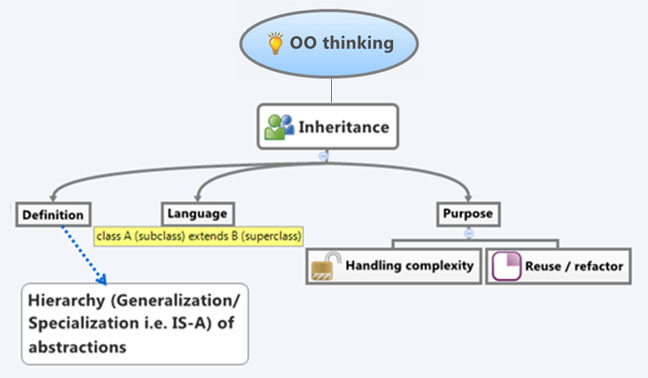
\includegraphics[scale=.3]{inheritance-oothinking.png}
 \end{center}
 \end{figure}
 Inheritance is the concept of a child class (sub class) automatically inheriting the variables and methods defined in its parent class (super class). 
 
\end{frame}

\begin{frame}{Inheritance}
 \texttt{Inheritance:}
 \begin{itemize}
  \item Inheritance can be defined as the process where one object acquires the properties of another. 
  \item The keyword used for inheritance in Java is ``extends''
  \item The relationship between two classes participating in Inheritance is ``is-a''
 \end{itemize}
\begin{block}{Example}
 \lstinline!class Mammal extends Animal!
\end{block}

\end{frame}

\begin{frame}{Inheritance}
 Use of Inheritance:
 \begin{itemize}
  \item Code Reusability
  \item Change Management
 \end{itemize}
 Types of Inheritance:
 \begin{itemize}
  \item Single or Simple Inheritance
  \item Multi-level Inheritance
  \item Hierarchial Inheritance
 \end{itemize}
\end{frame}


\begin{frame}{Inheritance}
 \begin{figure}[H]
 \begin{center}
   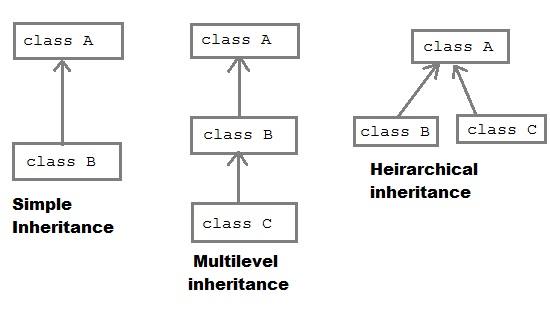
\includegraphics[scale=.5]{inheritance-levels.png}
 \end{center}
 \end{figure}
\end{frame}

\begin{frame}{Inheritance}
 \texttt{Multiple Inheritance:}
 \begin{figure}[H]
 \begin{center}
   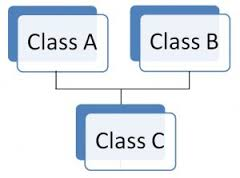
\includegraphics[scale=.35]{multiple-inheritance.png}
 \end{center}
 \end{figure}
 \begin{block}{Note}
  Java doesn't support Multiple Inheritance. In Java, a class cannot inherit more than one class.
 \end{block}
\end{frame}

\begin{frame}{Inheritance}
 \texttt{Deriving a Subclass:}
 
 To derive a child class, we use the extends keyword
 \begin{block}{Example}
  Suppose we have a parent class called Person. Then a subclass Student can be created as . . . 
 \end{block}
\end{frame}

\begin{frame}[fragile]{Inheritance}
\begin{figure}[H]
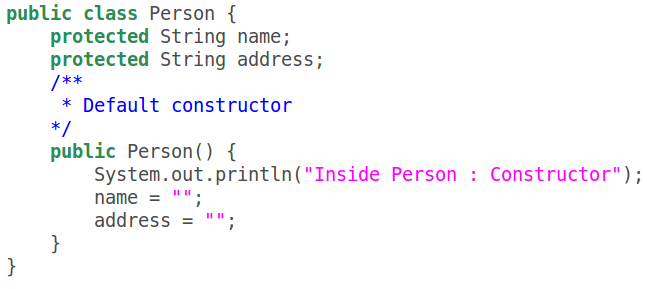
\includegraphics[scale=.4]{person-class.png}
\end{figure}
\begin{figure}[H]
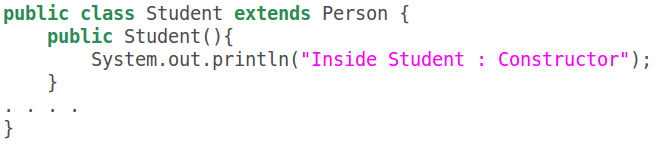
\includegraphics[scale=.4]{student-class.png}
\end{figure}
\end{frame}

\begin{frame}{Inheritance}
 What one can do in a Sub-class regarding Attributes
 \begin{itemize}
  \item The inherited attributes can be used directly, just like any other attributes
  \item You can declare new attributes in the subclass that are not in the super class
  \item You can declare an attribute in the subclass with the same name as the one in the super class, thus hiding it (not recommended)
   \end{itemize}
\end{frame}


\begin{frame}{Inheritance}
 What one can do in a Sub-class regarding Methods
 \begin{itemize}
  \item The inherited methods can be used directly as they are
  \item You can declare new methods in the subclass that are not in the super class
  \item You can write a new instance method in the subclass that has the same signature as the one in the super class, thus overriding it
 \end{itemize}

\end{frame}

\begin{frame}{Inheritance}
Need for ``super'' 

Let us consider the following  code snippet
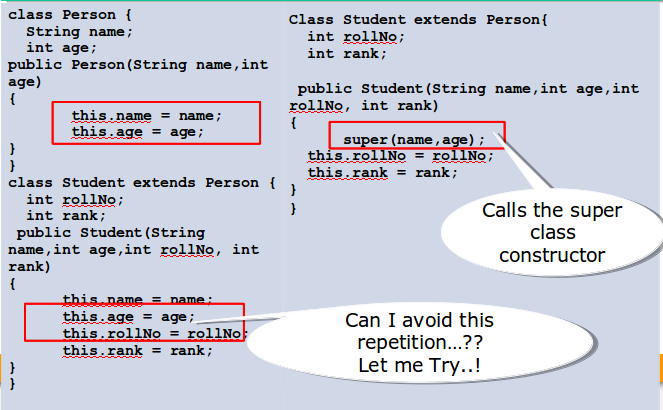
\includegraphics[scale=.4]{need-for-super.png}
 
\end{frame}


\begin{frame}{Inheritance}
What is ``super'' keyword?
\begin{itemize}
 \item A subclass can explicitly call a constructor of its super class using the super constructor call e.g.:\lstinline! super()!

 \item A super constructor call in the constructor of a subclass will result in the execution of relevant constructor from the super class, based on the arguments passed. 

Ex: \lstinline!super(10,20);!//it will invoke two-parameterized super class constructor
\end{itemize}
\end{frame}

\begin{frame}{Inheritance}
 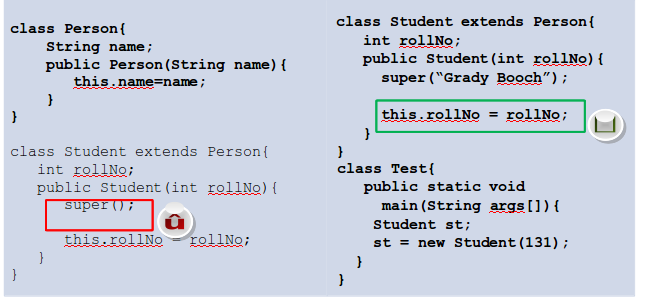
\includegraphics[height=3cm, width=11cm]{super-example.png}
 \begin{enumerate}
  \item By default, the compiler will insert a super() call in the sub-class constructor which calls the default constructor of the super-class. 
  \item If the super-class doesn’t have default constructor, we have to explicitly write a super() call in sub-class which matches with the constructor in super-class
 \end{enumerate}

\end{frame}

\begin{frame}{Inheritance}
Few things to remember when using the super constructor call: 
\begin{itemize}
 \item The \lstinline!super()! call must occur as the first statement in a constructor
 \item The \lstinline!super()! call can only be used in a constructor (not in ordinary methods)
 \item The Java compiler inserts \lstinline!super()! call as the first statement of sub class constructor if we don't provide it
\end{itemize}
Another use of super is to refer to members of the super class (just like the keyword ``\lstinline!this!'' ).
\end{frame}



\begin{frame}{Inheritance}
 When does super class constructor gets called ? 
 
 A subclass constructor invokes the constructor of the immediate superclass implicitly.
 
 In the below example the sub-class (Student) constuctor calls super-class (Person) constructor implictly.
 
 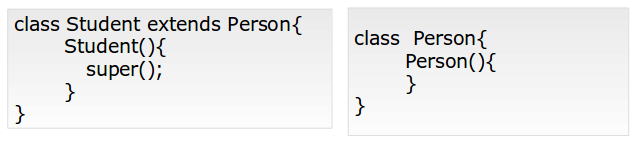
\includegraphics[scale=.5]{super-call.png}
\end{frame}

\begin{frame}{Inheritance}
 \textbf{Constructor  Chaining:}
 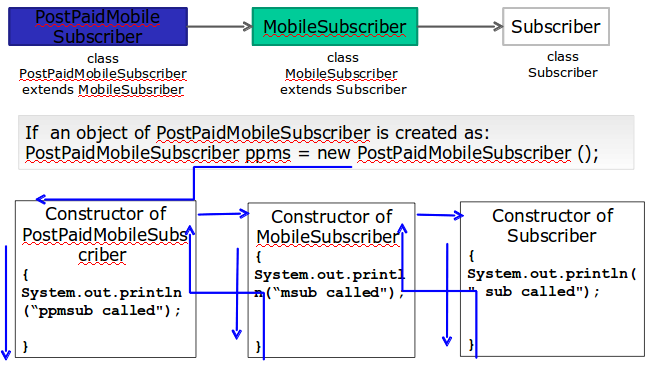
\includegraphics[scale=.5]{constructor-chaining.png}
\end{frame}


\begin{frame}[fragile]{Inheritance}
 Constructor Chaining in Inheritance
 \begin{lstlisting}[numbers=none, basicstyle=\tiny]
public class Subscriber {
    public Subscriber() {
        System.out.println("Subscriber  is called");
    }
}
public class MobileSubscriber extends Subscriber {
    public MobileSubscriber() {
        System.out.println("Mobile Subscriber is called");
    }
}
public class PostPaidMobileSubscriber extends MobileSubscriber {
    public PostPaidMobileSubscriber() {
        System.out.println("Postpaid mobile Subscriber is called");
    }
}
 \end{lstlisting}
\end{frame}

\begin{frame}[fragile]{Inheritance}
\begin{lstlisting}[numbers=none]
public class RunProgram {
    public static void main(String args[]) {
        PostPaidSubscriber ppsc = new PostPaidSubscriber();
    }
}
\end{lstlisting}
\begin{block}{Output}
Subscriber  is called

Mobile Subscriber is called

Postpaid mobile Subscriber is called
\end{block}
\end{frame}


\begin{frame}{Inheritance}
\begin{center}
    
\includegraphics[scale=0.5]{qa.png}
  \end{center}
  \end{frame}

\end{document}


